\documentclass[11pt,a4paper]{article}
\ifdefined\pdftexversion\pdfoutput=1\fi
\ifdefined\XeTeXrevision\PassOptionsToPackage{xetex}{hyperref}\fi
\usepackage[margin=24mm]{geometry}
\usepackage{amsmath,amssymb}
\usepackage{graphicx}
\usepackage{booktabs}
\usepackage{longtable}
\usepackage[table]{xcolor}
\usepackage{caption}
\usepackage[hidelinks]{hyperref}
\captionsetup{font=small,labelfont=bf,labelsep=period}
\setlength{\parindent}{0pt}
\setlength{\parskip}{.55em}
\definecolor{pass}{HTML}{176B45}
\definecolor{fail}{HTML}{8B1E1E}
\newcolumntype{L}[1]{>{\raggedright\arraybackslash}p{#1}}
\newcommand{\PASS}{\textcolor{pass}{\textbf{pass}}}
\newcommand{\FAIL}{\textcolor{fail}{\textbf{fail}}}

\title{What was rederived, what was reproduced, and what was only called\\[.35em]
\large A verification record for the finite-coupling extremality-shift calculation}
\author{}
\date{28 September 2026}

\begin{document}
\maketitle
\thispagestyle{empty}

\begin{abstract}
\noindent
This is not a physics paper; it is an audit trail. It states, claim by claim,
which parts of the accompanying calculation were derived here, which were
computed here and checked against something external, which were copied from a
paper and verified against that paper, and which were simply used on the
author's authority. Of 58 entries,
47 carry a machine-checked verdict and
11 are listed as called and not reproduced.
0 checks fail.
The external anchors are the Myers--Perry solution in the vacuum limit, the
Boulware--Deser solution at finite coupling and zero spin, the perturbative
potential of Wu and L\"u at zero coupling, the extremal near-horizon branch of
Brihaye, Kleihaus, Kunz and Radu at finite coupling, and the extremality shift
of Ma, Li and L\"u. Everything is regenerated by
\texttt{work/verification\_suite.py}, which is what produced the tables below.
\end{abstract}

\section*{How to read this}

Four kinds of entry appear, and the distinction between them is the reason the
document exists. A calculation that agrees with itself has shown nothing; the
question is always what it was tested against, and with what.

\begin{description}
\item[Rederived analytically.] Redone here symbolically, with the difference
asserted to be exactly zero. These need no tolerance because nothing numerical
enters: either the expressions are identical or they are not.
\item[Reproduced numerically.] Produced by the spectral solver and compared with
a closed form or a published equation. Each carries the tolerance its assertion
used, and figures~\ref{fig:fig-myers-perry}--\ref{fig:fig-near-horizon} draw
the deviation against that tolerance so the margin is visible rather than
asserted.
\item[Transcription checked against the source.] Every convention this work
imports --- a coupling normalisation, a charge normalisation, a factor in a
near-horizon metric --- read back from the source PDF. These were previously the
weakest link: the manuscript's own referee record listed the literature
attributions as unverified because no source PDFs were present. They now are,
under \texttt{papers/}, and the checks below read them.
\item[Called, not reproduced.] Used and not re-derived. Listing these is the
only way the three categories above mean anything.
\end{description}

\section*{The three conversions that everything else depends on}

Three numbers relate this work's conventions to the literature, and a mistake in
any of them would move every finite-coupling comparison without breaking any
internal check. Each is now verified twice, by independent routes.

\paragraph{The coupling.} The source writes its action as
$I=(16\pi G)^{-1}\int\!\sqrt{-g}\,(R+\tfrac{\alpha_{\rm ref.}}{4}\mathcal L_{\rm GB})$
while this work writes $R+\alpha\mathcal L_{\rm GB}$, so
$\alpha_{\rm ref.}=4\alpha$. That is read directly from eq.~(2.1) of
arXiv:1010.0860. Independently, the ratio of the Gauss--Bonnet piece of the
published entropy~(3.10) to its Einstein piece equals the ratio our
Jacobson--Myers form gives \emph{only} if $\alpha_{\rm ref.}=4\alpha$; that
is checked symbolically. Two routes, one answer.

\paragraph{The angular momentum.} The source's $J$ is the momentum in
\emph{each} plane, not the total, which is the sentence introducing its
eq.~(3.6). Its normalisations $E=-3V_3U/16\pi G$ and $J=V_3W/8\pi G$ with
$V_3=2\pi^2$ reduce to the $-3\pi U/8$ and $\pi W/4$ used here.

\paragraph{The near-horizon $k$.} The source's near-horizon metric carries
$\sigma_3+2kr\,\mathrm{d}t$ where this work writes $\sigma_3+kr\,\mathrm{d}t$,
so $k=2k_{\rm ref.}$ and, since $J=\partial E/\partial k$,
$J_{\rm ref.}=2J$. This is what reconciles the source's
$S_{\rm ext}=\pi J_{\rm ref.}$ at zero coupling with the
$S_{\rm ext}=2\pi J$ obtained here, and both with extremal Myers--Perry,
$S=2\pi^2a^3$ and $J=\pi a^3$. Without the factor this would look like a
discrepancy of two; with it, the three statements are one statement.

\section*{The ledger}

\subsection*{Rederived analytically}
Redone here with sympy and the difference asserted to vanish identically. No tolerance and no solver output enters.

\begin{longtable}{@{}L{.38\textwidth}L{.24\textwidth}rrc@{}}
\toprule
claim & source & result & tolerance & verdict \\
\midrule\endhead
Psi\_static = (3pi/4)(4a-3)/(1+4a) from dM/da - T dS/da & Boulware-Deser charges; manuscript eq. (15) & -- & -- & \PASS \\
Psi\_static -> -9pi/4 as alpha -> 0 & manuscript eq. (15) & -- & -- & \PASS \\
Psi\_static changes sign at alpha/r\_H\textasciicircum{}2 = 3/4 & manuscript sec. 4.1 & -- & -- & \PASS \\
Smarr 2M = 3TS + 2*alpha*Psi closes on Boulware-Deser at J=0 & manuscript eq. (8) on eq. (14) & -- & -- & \PASS \\
static t\_H = sqrt(1+2a)/(1+4a) follows from eq. (10) & manuscript sec. 2.3 & -- & -- & \PASS \\
Euler on the listed weights gives 2M = 3TS + 3 sum(Omega\_i J\_i) + 2 alpha Psi & manuscript eq. (8) & -- & -- & \PASS \\
its equal-spin case is the printed 2M = 3TS + 6 Omega\_H J + 2 alpha Psi & manuscript eq. (8) & -- & -- & \PASS \\
differentiated Smarr minus twice the first law is the printed Gibbs-Duhem constraint & manuscript sec. 3.1 & -- & -- & \PASS \\
q = r\_H Omega\_H = a/r\_H from Omega\_H = a/(r\_+\textasciicircum{}2+a\textasciicircum{}2), r\_H\textasciicircum{}2 = r\_+\textasciicircum{}2+a\textasciicircum{}2 & manuscript eq. (9) & -- & -- & \PASS \\
u = q\textasciicircum{}2/(1-q\textasciicircum{}2) equals a\textasciicircum{}2/r\_+\textasciicircum{}2 & manuscript eq. (9) & -- & -- & \PASS \\
equal-spin Myers-Perry is extremal at r\_+ = a (d mu / d r\_+ = 0) & Myers-Perry horizon function & -- & -- & \PASS \\
hence extremality sits at q = 1/sqrt(2) & manuscript sec. 2.1 & -- & -- & \PASS \\
M = 3pi r\_H\textasciicircum{}2/[8(1-q\textasciicircum{}2)] is the same as 3 pi mu\_MP / 8 & manuscript appendix A & -- & -- & \PASS \\
Psi\_0(u=0) = -9pi/4, matching the alpha->0 limit of Psi\_static & manuscript eq. (17) against eq. (15) & -- & -- & \PASS \\
Psi\_0(u=1) = pi, matching the published linear-order slope & manuscript eq. (17) against arXiv:2009.00015 & -- & -- & \PASS \\
Psi\_0 sign zero at q = 7-2sqrt(10) mapped through eq. (9) & manuscript sec. 4.2 & $6.35\times10^{-1}$ & $1.00\times10^{-9}$ & \PASS \\
our metric ansatz is identically eq. (2.8) of 1010.0860 with g = r\textasciicircum{}2 & manuscript eq. (4) against arXiv:1010.0860 eq. (2.8) & -- & -- & \PASS \\
the published entropy (3.10) equals our Jacobson-Myers form iff alpha\_paper = 4 alpha & manuscript eq. (7) against arXiv:1010.0860 eq. (3.10) & -- & -- & \PASS \\
dS/dalpha at fixed (M,J) equals -Psi/T, from the extended first law & manuscript sec. 3.2 & -- & -- & \PASS \\
\bottomrule
\end{longtable}

\subsection*{Reproduced numerically}
Computed by this project's solver and compared against a closed form or a published equation. Each carries the tolerance its assertion used.

\begin{longtable}{@{}L{.38\textwidth}L{.24\textwidth}rrc@{}}
\toprule
claim & source & result & tolerance & verdict \\
\midrule\endhead
the alpha=0 mass reproduces the Myers-Perry closed form & Myers-Perry, M = 3 pi r\_H\textasciicircum{}2/[8(1-q\textasciicircum{}2)] & $3.27\times10^{-13}$ & $1.00\times10^{-10}$ & \PASS \\
the alpha=0 horizon squashing reproduces the Myers-Perry 1/(1-q\textasciicircum{}2) & Myers-Perry & $8.30\times10^{-14}$ & $1.00\times10^{-8}$ & \PASS \\
the static mass reproduces the Boulware-Deser closed form at finite coupling & Boulware-Deser & $3.20\times10^{-11}$ & $1.00\times10^{-8}$ & \PASS \\
the static temperature reproduces the Boulware-Deser closed form at finite coupling & Boulware-Deser & $1.08\times10^{-13}$ & $1.00\times10^{-8}$ & \PASS \\
the static entropy reproduces the Boulware-Deser closed form at finite coupling & Boulware-Deser & $1.00\times10^{-16}$ & $1.00\times10^{-8}$ & \PASS \\
the static potential reproduces the Boulware-Deser closed form at finite coupling & Boulware-Deser & $2.60\times10^{-9}$ & $1.00\times10^{-8}$ & \PASS \\
the alpha=0 response reproduces the published perturbative potential & arXiv:2405.04576 eq. (33), mapped by manuscript eq. (17) & $2.86\times10^{-8}$ & $1.00\times10^{-6}$ & \PASS \\
our near-horizon solution satisfies published eq. (4.11) as printed & arXiv:1010.0860 eq. (4.11) & $9.17\times10^{-14}$ & $1.00\times10^{-10}$ & \PASS \\
our near-horizon solution satisfies published eq. (4.12) as printed & arXiv:1010.0860 eq. (4.12) & $6.66\times10^{-16}$ & $1.00\times10^{-10}$ & \PASS \\
the near-horizon branch gives S\_ext = 2 pi J at alpha=0, the extremal Myers-Perry value & Myers-Perry; arXiv:1010.0860 eq. (4.13) after k\_paper = k/2 & $1.11\times10^{-12}$ & $1.00\times10^{-10}$ & \PASS \\
the extrapolated bulk entropy reproduces the near-horizon curve at finite coupling & arXiv:1010.0860 sec. 4.2 & $4.06\times10^{-6}$ & $1.00\times10^{-4}$ & \PASS \\
the extrapolated mu(0) reproduces the published (3/2) pi\textasciicircum{}(1/3) & arXiv:2009.00015 & $4.56\times10^{-11}$ & $1.00\times10^{-8}$ & \PASS \\
the extrapolated Psi\_ext(0) reproduces the published pi & arXiv:2009.00015 & $1.19\times10^{-7}$ & $1.00\times10^{-5}$ & \PASS \\
the vacuum extremal state returns the normalisation value j = 1 & arXiv:2303.12471 scaled spin & $3.11\times10^{-11}$ & $1.00\times10^{-6}$ & \PASS \\
the Smarr relation closes on every accepted rotating solution & manuscript eq. (8) & $1.64\times10^{-7}$ & $1.00\times10^{-6}$ & \PASS \\
the first law closes in the spin direction at fixed coupling & manuscript eq. (2) & $1.35\times10^{-8}$ & $1.00\times10^{-6}$ & \PASS \\
every accepted state satisfies G + alpha H = 0 off the solver grid & Einstein-Gauss-Bonnet field equations & $9.76\times10^{-9}$ & $1.00\times10^{-8}$ & \PASS \\
the extremal intercept survives two coarser radial resolutions at every coupling & this work, resolution study & $1.50\times10^{-3}$ & $1.00\times10^{0}$ & \PASS \\
\bottomrule
\end{longtable}

\subsection*{Transcription checked against the source}
A convention, normalisation or formula this work takes from a paper, checked against the text of that paper as downloaded in \texttt{papers/}.

\begin{longtable}{@{}L{.38\textwidth}L{.24\textwidth}rrc@{}}
\toprule
claim & source & result & tolerance & verdict \\
\midrule\endhead
the source action carries alpha/4 on L\_GB, so alpha\_paper = 4 alpha & arXiv:1010.0860 eq. (2.1) & -- & -- & \PASS \\
the source charges are E = -3 V\_3 U/16 pi G and J = V\_3 W/8 pi G with V\_3 = 2 pi\textasciicircum{}2 & arXiv:1010.0860 eq. (3.6) & -- & -- & \PASS \\
the source J is the momentum in each plane, not the total & arXiv:1010.0860 sec. 3.2 & -- & -- & \PASS \\
the source near-horizon metric carries 2k, so our k is twice theirs & arXiv:1010.0860 eq. (4.6) & -- & -- & \PASS \\
the source entropy has an Einstein piece and a GB piece of the printed form & arXiv:1010.0860 eq. (3.10) & -- & -- & \PASS \\
the source quotes an outer ergosurface radius at the coupling we compare with & arXiv:1010.0860 sec. 4.1 & -- & -- & \PASS \\
the published extremal mass is M = (3/2) pi\textasciicircum{}(1/3) J\textasciicircum{}(2/3) + pi alpha + O(alpha\textasciicircum{}2) & arXiv:2009.00015 & -- & -- & \PASS \\
the source uses the same 1/16 pi action normalisation, with G = 1 & arXiv:2405.04576 eq. (25) & -- & -- & \PASS \\
their Delta M = (D-4) Delta G at D=5 with equal spins is exactly our eq. (17) & arXiv:2405.04576 eq. (33) & -- & -- & \PASS \\
the source treats a general quadratic-curvature correction on a Ricci-flat background & arXiv:2405.04576 & -- & -- & \PASS \\
\bottomrule
\end{longtable}

\subsection*{Called, not reproduced}
Used on the authority of the source. Listed so that it cannot be mistaken for anything above.

\begin{longtable}{@{}L{.30\textwidth}L{.22\textwidth}L{.42\textwidth}@{}}
\toprule
what & source & status \\
\midrule\endhead
The Myers-Perry solution itself & Myers \& Perry, Annals Phys. 172 (1986) 304 & Its closed forms are used as an oracle and every one of them is checked against our solver, but the solution is not rederived here. Not on arXiv, so no PDF is in papers/. \\
The Boulware-Deser solution itself & Boulware \& Deser, PRL 55 (1985) 2656 & Same status: the closed forms for M, T and S are the oracle for the static limit, and we differentiate them to get Psi, but the solution is not rederived. Not on arXiv. \\
Lovelock's theorem & Lovelock, J. Math. Phys. 12 (1971) 498 & Cited for the field equations being second order. Not reproduced. Not on arXiv. \\
The Wald entropy formula & arXiv:gr-qc/9307038, arXiv:gr-qc/9403028 & The Noether-charge form is cited, not derived. Its value on this horizon is checked against the independent derivation in arXiv:1010.0860. \\
The Jacobson-Myers form for Lovelock horizons & arXiv:hep-th/9305016 & Cited as the form Wald entropy takes here; the resulting entropy is then verified numerically against the published near-horizon branch. \\
Sen's entropy function formalism & arXiv:0708.1270 & The formalism is cited. Our use of it is rederived symbolically and its solution checked against the full field equations component by component, but the formalism itself is not re-justified. \\
The domain bounds x < 1 and j <= 1 & arXiv:2303.12471 & Quoted and compared against, not rederived. Our samples lie inside them. \\
The Goon-Penco universality argument & arXiv:1909.05254 & Only the first-law identity is used, and that is rederived here. The universality claim itself is cited and not tested. \\
Causality constraints on higher-curvature couplings & arXiv:1407.5597 & Cited in the discussion as a reason to separate the classical truncation from an ultraviolet completion. Nothing is computed from it. \\
The extended first law for Lovelock couplings & arXiv:1005.5053, arXiv:2404.16981 & Cited as the source of the Psi dalpha term. The term is then used and its consequences checked internally, but the covariant-phase-space derivation is not repeated. \\
The outer ergosurface radius 1.104 at alpha = 1/2 & arXiv:1010.0860 & Compared against and does NOT reproduce: our reconstruction gives 1.102101. Unresolved; recorded in the manuscript discussion as an open point. \\
\bottomrule
\end{longtable}


\section*{Sources held locally}

Every paper the calculation leans on that exists on arXiv is in
\texttt{papers/}, and the transcription checks above read them from there. The
three pre-arXiv sources --- Myers and Perry (1986), Boulware and Deser (1985)
and Lovelock (1971) --- are not available that way and are listed as called.

\begin{center}
\small
\begin{tabular}{@{}lr@{}}
\toprule
file & size \\
\midrule
\texttt{0708.1270-sen-entropy-function-attractors.pdf} & 1835\,kB \\
\texttt{1005.5053-kastor-ray-traschen-smarr-lovelock.pdf} & 262\,kB \\
\texttt{1010.0860-brihaye-kleihaus-kunz-radu-equal-spin-egb-d5.pdf} & 396\,kB \\
\texttt{1306.2517-kunduri-lucietti-near-horizon-classification.pdf} & 883\,kB \\
\texttt{1407.5597-camanho-edelstein-maldacena-zhiboedov-causality.pdf} & 706\,kB \\
\texttt{1901.11535-reall-santos-higher-derivative-kerr-thermodynamics.pdf} & 474\,kB \\
\texttt{1909.05254-goon-penco-entropy-extremality-relation.pdf} & 171\,kB \\
\texttt{2009.00015-ma-li-lu-d5-egb-mass-angular-momentum-extremality.pdf} & 281\,kB \\
\texttt{2303.12471-kleihaus-kunz-radu-phases-rotating-d5-egb.pdf} & 301\,kB \\
\texttt{2404.16981-neri-liberati-covariant-phase-space-lanczos-lovelock.pdf} & 877\,kB \\
\texttt{2405.04576-wu-lu-quadratic-curvature-rotating-thermodynamics.pdf} & 301\,kB \\
\texttt{2512.23797-ma-lu-quadratic-curvature-correction-5d-myers-perry.pdf} & 245\,kB \\
\texttt{gr-qc-9307038-wald-black-hole-entropy-noether-charge.pdf} & 142\,kB \\
\texttt{gr-qc-9403028-iyer-wald-noether-charge-dynamical-entropy.pdf} & 307\,kB \\
\texttt{hep-th-0601001-arkani-hamed-motl-nicolis-vafa-weak-gravity.pdf} & 213\,kB \\
\texttt{hep-th-0606100-kats-motl-padi-higher-order-extremal-mass-charge.pdf} & 174\,kB \\
\texttt{hep-th-9305016-jacobson-myers-entropy-higher-curvature.pdf} & 134\,kB \\
\bottomrule
\end{tabular}
\end{center}

\section*{What this record does not establish}

Agreement with an external result bounds the error at the point of comparison
and nowhere else. The vacuum and static checks are exact but sit at the edges of
the family --- zero coupling and zero spin --- and the near-horizon check
constrains the entropy, not the mass. No external result exists for the rotating
mass at finite coupling, which is precisely the quantity the accompanying
manuscript reports; that number rests on the solver, its convergence behaviour
and the zero-temperature extrapolation, and on nothing published. The tolerances
quoted here are the ones the assertions used, chosen to be loose enough to pass
reliably and not as estimates of the accuracy achieved: the achieved deviations
are typically several orders of magnitude smaller, which is what the lower
panels of the figures show.

\begin{figure}[p]
 \centering
 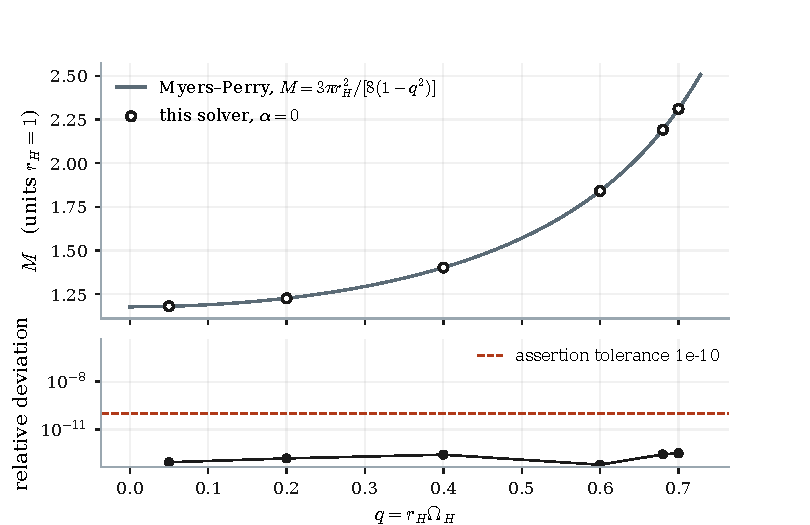
\includegraphics[width=.92\textwidth]{figures/fig-myers-perry.pdf}
 \caption{\textbf{The vacuum limit against Myers--Perry.} Upper: the mass of the solver's $\alpha=0$ solutions against the closed form $M=3\pi r_H^2/[8(1-q^2)]$, which follows from $3\pi\mu/8$ and the coordinate map $r^2=\rho^2+a^2$ rederived in this report. Lower: the relative deviation, against the tolerance the assertion used. The comparison runs to $q=0.7$, past the vacuum extremal spin $1/\sqrt2$ being approached.}
 \label{fig:fig-myers-perry}
\end{figure}
\begin{figure}[p]
 \centering
 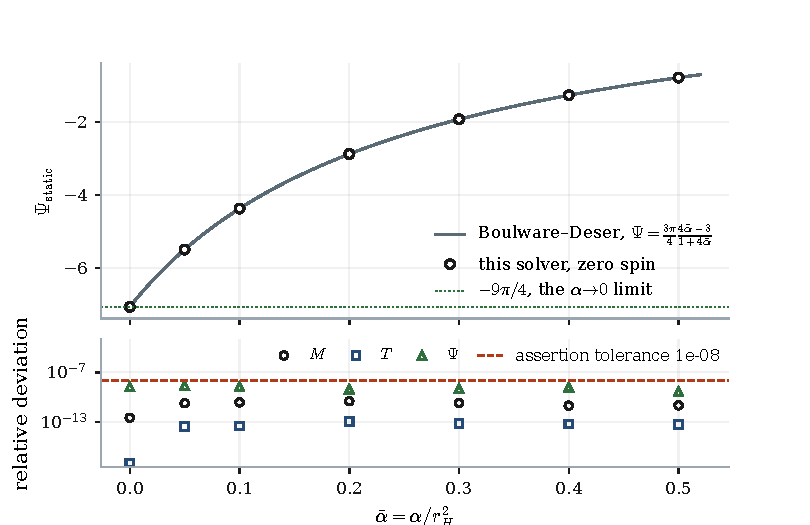
\includegraphics[width=.92\textwidth]{figures/fig-boulware-deser.pdf}
 \caption{\textbf{The static limit against Boulware--Deser, at finite coupling.} Upper: the potential $\Psi$ measured at zero spin against the closed form derived in this report by differentiating the Boulware--Deser charges. This is the one exact check available at $\alpha\neq0$. The dotted line is the $\alpha\to0$ value $-9\pi/4$, which the independent perturbative formula also returns. Lower: relative deviations in $M$, $T$ and $\Psi$. The entropy is reproduced to machine precision and is omitted from the lower panel for that reason.}
 \label{fig:fig-boulware-deser}
\end{figure}
\begin{figure}[p]
 \centering
 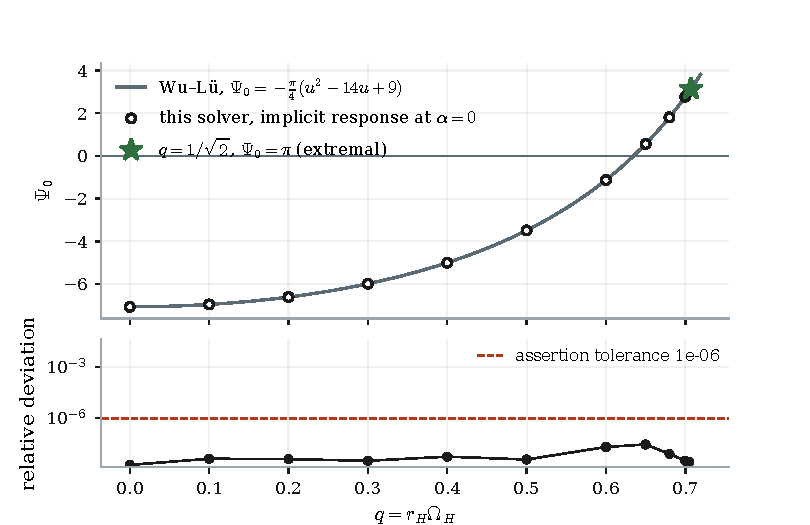
\includegraphics[width=.92\textwidth]{figures/fig-perturbative.pdf}
 \caption{\textbf{The zero-coupling response against the published perturbative potential.} Upper: the implicit numerical response evaluated on the Myers--Perry background against $\Psi_0(q)$, which this report re-derives by specialising the general-$D$ result of Wu and L\"u to $D=5$ with equal spins rather than by copying it. The star marks the extremal endpoint $\Psi_0=\pi$, which is the published linear-order extremality shift and was not used in obtaining the curve. Lower: relative deviation.}
 \label{fig:fig-perturbative}
\end{figure}
\begin{figure}[p]
 \centering
 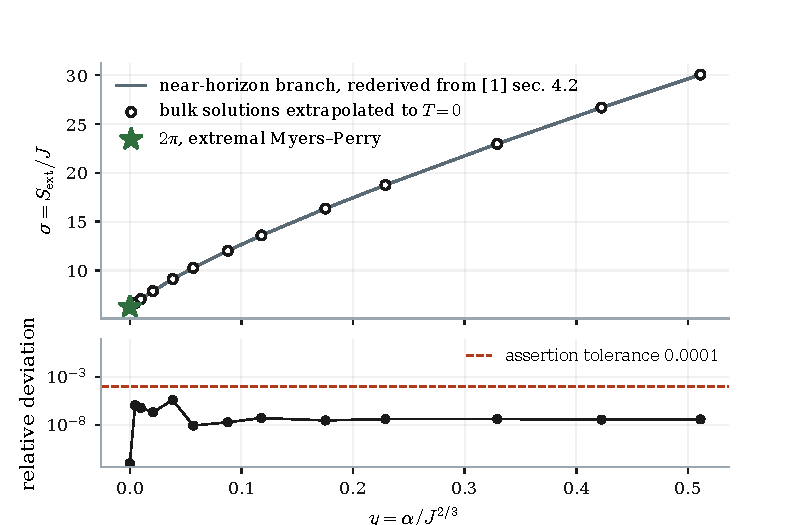
\includegraphics[width=.92\textwidth]{figures/fig-near-horizon.pdf}
 \caption{\textbf{The extremal entropy against the published near-horizon branch.} Upper: $\sigma=S_\mathrm{ext}/J$ from the near-horizon entropy function, rederived here and checked against eqs.~(4.11) and~(4.12) of arXiv:1010.0860 in the paper's own variables, against the zero-temperature extrapolation of the bulk solutions. The star is the extremal Myers--Perry value $2\pi$. Lower: relative difference between the two routes.}
 \label{fig:fig-near-horizon}
\end{figure}

\vfill
\noindent\rule{\textwidth}{.4pt}\par
\footnotesize
Generated by \texttt{verification-report/build\_report.py} from
\texttt{results/verification-ledger.json}. Environment:
Linux-6.8.0-142-generic-x86\_64-with-glibc2.39, Python 3.12.3, NumPy
1.26.4, SymPy 1.12.

\end{document}
